\documentclass[10pt, letterpaper]{paper}
\usepackage{graphicx}
\usepackage{amsmath}
\usepackage{float}

\title{ Operations Research Test 1 }
\author{ Timothy Schwieg }
\date{ October 4 2017 }

\begin{document}

\maketitle

\section*{Question 1 }
\subsection*{a.}

\begin{equation*}
\begin{alignedat}{3}
&\text{max }&80x_1 + 100x_2&\\
&\text{s.t. } &20x_1 + 40x_2  &\leq 1000\\
& &60x_1 + 40x_2  &\leq 1240\\
& &12x_1 + 4x_2 &\leq 200\\
& &x_1, x_2 &\geq 0
\end{alignedat}
\end{equation*}

Adding in slack variables, this becomes:

\begin{equation*}
\begin{alignedat}{3}
&\text{max }&80x_1 + 100x_2&\\
&\text{s.t. } &20x_1 + 40x_2 + s_1  &= 1000\\
& &60x_1 + 40x_2 + s_2 &= 1240\\
& &12x_1 + 4x_2 + s_3 &= 200\\
& &x_1, x_2, s_1, s_2, s_3 &\geq 0
\end{alignedat}
\end{equation*}

Putting in Tableau form:

\[
	\left[ {\begin{array}{cccccc|c}
	Z & x_1 & x_2 & s_1 & s_2 & s_3 & RHS\\ \cline{1-7}
	1 & -80 & -100& 0 & 0 & 0 & 0 \\
	0 & 20 & 40 & 1 & 0 & 0 &1000\\
	0 & 60 & 50 & 0& 1 & 0 & 1240\\
	0 & 12 & 4 & 0 & 0 & 1 & 200 \\
	\end{array} } \right]
\]

\[
	\left[ {\begin{array}{cccccc|c}
	Z & x_1 & x_2 & s_1 & s_2 & s_3 & RHS\\ \cline{1-7}
	1 & -30 & 0 & \frac{5}{2} & 0 & 0 & 2500 \\
	0 & \frac{1}{2} & 1 & \frac{1}{40} & 0 & 0 &25\\
	0 & 40 & 0 & -1 & 1 & 0 & 240\\
	0 & 10 & 0 & \frac{-1}{10} & 0 & 1 & 100 \\
	\end{array} } \right]
\]

\[
	\left[ {\begin{array}{cccccc|c}
	Z & x_1 & x_2 & s_1 & s_2 & s_3 & RHS\\ \cline{1-7}
	1 & 0 & 0 & \frac{7}{4} & \frac{3}{4} & 0 & 2680 \\
	0 & 0 & 1 & \frac{3}{80} & \frac{-1}{80} & 0 &22\\
	0 & 1 & 0 & \frac{-1}{40} & \frac{1}{40} & 0 & 6\\
	0 & 0 & 0 & \frac{3}{20} & \frac{-1}{4} & 1 & 40 \\
	\end{array} } \right]
\]

We can see that the optimal solution is: 2680 obtained where $x_1 = 6,x_2 = 22$.

\subsection*{b.}
Note that since $s_3 = 40$, there is slack in the third constraint, and therefore we are not using all the workers. This indicates that there are 40 worker-hours not being utilized, and HR should lay off one worker as only 4 are required.

\subsection*{c.}
We would like to relax the costraint on the resource with the highest shadow price, and would therefore like to hire an additional worker in Cutting, as
$\frac{7}{4} > \frac{3}{4}$.

\subsection*{d.}
Forming the RHS Tableau:

\[
	\left[ {\begin{array}{cccccc|c|cccc}
	Z & x_1 & x_2 & s_1 & s_2 & s_3 & RHS & d_1 & d_2 & d_3\\ \cline{1-10}
	1 & 0 & 0 & \frac{7}{4} & \frac{3}{4} & 0 & 2680 & \frac{7}{4} & \frac{3}{4} & 0\\
	0 & 0 & 1 & \frac{3}{80} & \frac{-1}{80} & 0 &22& \frac{3}{80} & \frac{-1}{80} & 0\\
	0 & 1 & 0 & \frac{-1}{40} & \frac{1}{40} & 0 & 6 & \frac{-1}{40} & \frac{1}{40} & 0\\
	0 & 0 & 0 & \frac{3}{20} & \frac{-1}{4} & 1 & 40 & \frac{3}{20} & \frac{-1}{4} & 1\\
	\end{array} } \right]
\]
Note that since only the workers in the sewing department change: $d_1 = d_3 = 0$
\newline
We can see from this that: 
\begin{eqnarray*}
22 - \frac{1}{80} d_2 &\geq 0\\
6 + \frac{1}{40} d_2 &\geq 0\\
40 - \frac{1}{4} d_2 &\geq 0\\
\end{eqnarray*}
This yeilds: 
\begin{eqnarray*}
d_2 &\leq 1760\\
d_2 &\geq -240\\
d_2 &\leq 160\\
\end{eqnarray*}

From this it is plain that: $d_2 \in [-240,160]$ and that we can remove as many as 6, and add as many as 4 workers without altering the form of the final tableau.

\subsection*{e.}
Forming the Objective function tableau:

\[
	\left[ {\begin{array}{ccccccc|c}
	 & 1 & d_1 &d_2 & 0 &0 &0& 0\\
	 & Z & x_1 & x_2 & s_1 & s_2 & s_3 & RHS\\ \cline{1-7}
	1& 1 & 0 & 0 & \frac{7}{4} & \frac{3}{4} & 0 & 2680 \\
	d_1 & 0 & 0 & 1 & \frac{3}{80} & \frac{-1}{80} & 0 &22\\
	d_2 & 0 & 1 & 0 & \frac{-1}{40} & \frac{1}{40} & 0 & 6\\
	0 & 0 & 0 & 0 & \frac{3}{20} & \frac{-1}{4} & 1 & 40 \\
	\end{array} } \right]
\]

Noting that if only the price of shirts changes, then $d_2 = 0$, our feasibility constraints are:

\begin{eqnarray*}
\frac{7}{4} + \frac{3}{80} d_1 &\geq 0 \\
\frac{3}{4} - \frac{1}{80} d_1 &\geq 0\\
\end{eqnarray*}

This reduces to:
\begin{eqnarray*}
d_1 &\leq 60\\
d_1 &\geq \frac{-140}{3}\\
\end{eqnarray*}

We can see that $d_1 = 25$ is within this range, and will therefore not change the optimal solution.
\newline
The new maximum will be: $6*105 + 22*100 = 2830$.

\section*{Question 2}
\subsection*{a.}
The dual is given by:
\begin{equation*}
\begin{alignedat}{3}
&\text{min \quad }&5\lambda_1 + 8\lambda_2&\\
&\text{s.t. } &\lambda_1 + 2\lambda_2  &\leq 3\\
& &2\lambda_1 + 3\lambda_2 &\geq 4\\
& &\lambda_1 + \lambda_2 &\geq 1\\
& &2\lambda_1 + 3\lambda_2 &\leq 5\\
& &\lambda_1, \lambda_2 &\geq 0
\end{alignedat}
\end{equation*}


\subsection*{b.}
Solving it graphically:

\begin{figure}[H]
\centering
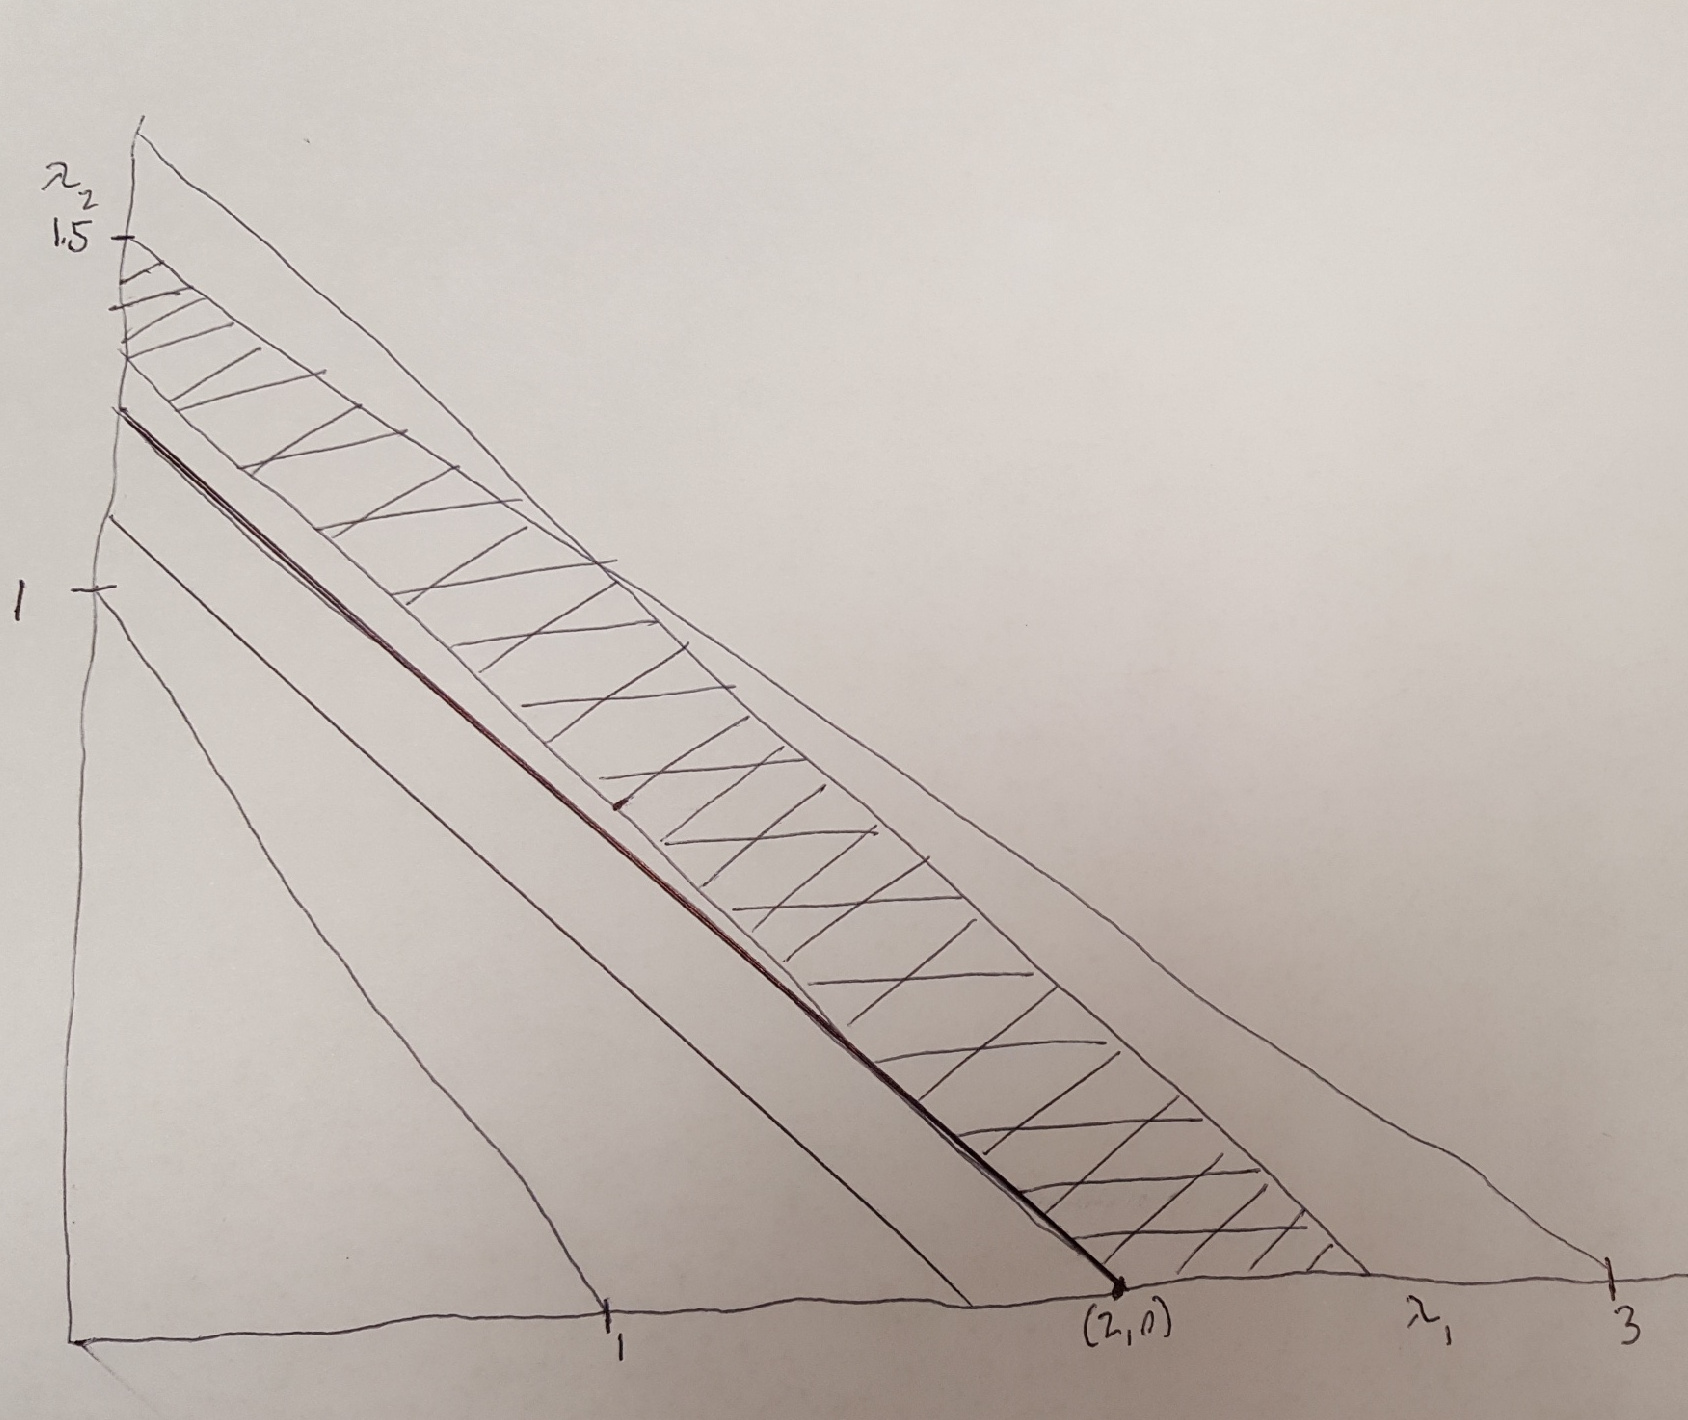
\includegraphics[width=1.0\textwidth]{shittygraph.jpeg}
\end{figure}

Note that the feasible set is the cross-hatched area, and the objective contour with the minimum is bolded.

We can see that the optimal solution is located at: $\lambda_1 = 2, \lambda_2 = 0$
\subsection*{c.}
Via Complementary slackness we arrive at the following equations:
\begin{eqnarray*}
(5 - x_1 - 2x_2 -x_3 - 2x_4 )\lambda_1 &= 0\\
(8 - 2x_1 - 3x_2 -x_3 -3x_4)\lambda_2 &= 0\\
(3 - \lambda_1- 2\lambda_2) x_1 &= 0\\
(4- 2\lambda_1 - 3\lambda_2 )x_2 &= 0\\
(1 - \lambda_1 - \lambda_2 )x_3 &= 0\\
(5 - 2\lambda_1 - 3\lambda_2)x_4 &= 0\\
\end{eqnarray*}
Plugging in: $\lambda_1 = 2, \lambda_2 = 0$.

\begin{eqnarray*}
5 - x_1 - 2x_2 - x_3 - 2x_4 &= 0 \\
0 &= 0\\
x_1 &= 0\\
0 &= 0\\
-x_3 &= 0\\
x_4 &= 0\\
\end{eqnarray*}
We are left with only $x_2$ unknown, and can solve for it with the first equation.
\newline
$x_1 = 0, x_2 = \frac{5}{2}, x_3 = 0,x_4 = 0$.

\section*{Question 3.}

\subsection*{a.}

\begin{figure}[H]
\centering
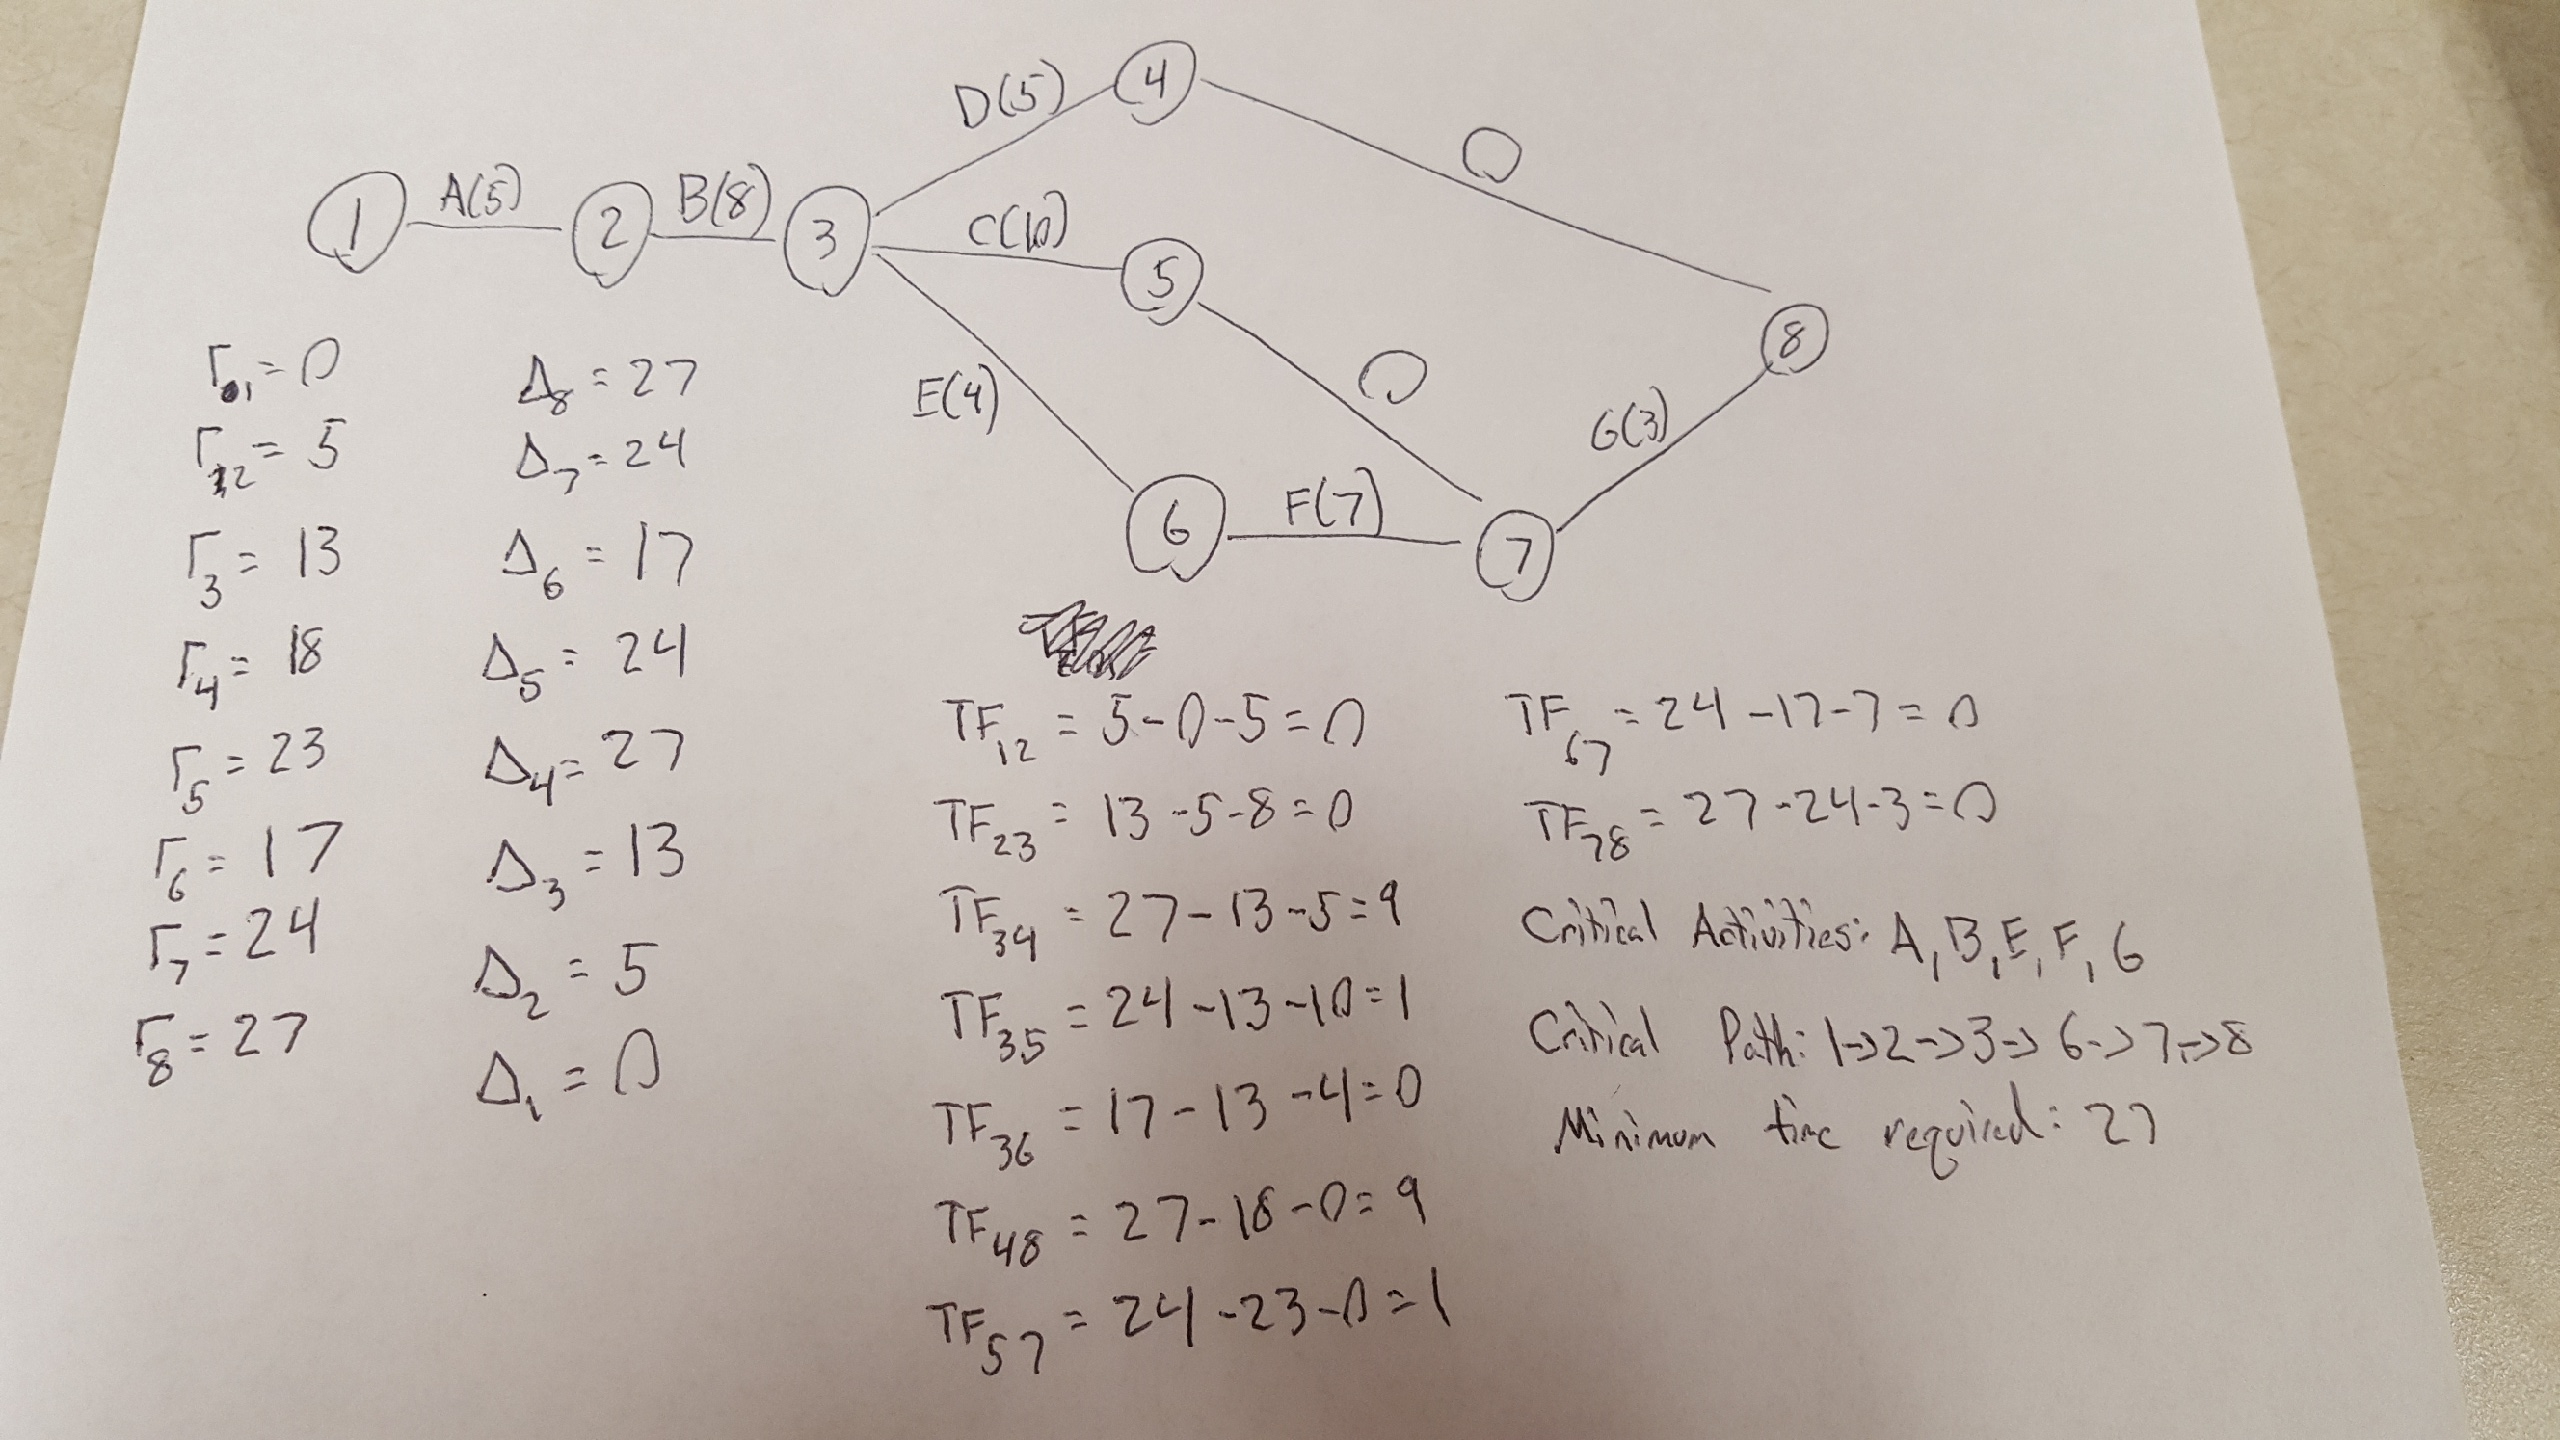
\includegraphics[width=1.0\textwidth]{ProjectNodes.jpeg}
\end{figure}


\subsection*{b.}
This can be written as a linear program of the form:
\begin{equation*}
\begin{alignedat}{3}
&\text{min }&30d_A + 15d_B + 20d_C + 40d_D + 20d_E + 30d_F + 40d_C&\\
&\text{s.t. } &t_8 - t_1  &\leq 19\\
& &t_8 - t_7 + d_G &\geq 3\\
& &t_7 - t_6 + d_F &\geq 7\\
& &t_6 - t_3 + d_E &\geq 4\\
& &t_5 - t_3 + d_C &\geq 10\\
& &t_4 - t_3 + d_D &\geq 5\\
& &t_3 - t_2 + d_B &\geq 8\\
& &t_2 - t_1 + d_A &\geq 5\\
& &d_A &\leq 2\\
& &d_B &\leq 3\\
& &d_C &\leq 1\\
& &d_D &\leq 2\\
& &d_E &\leq 2\\
& &d_F &\leq 3\\
& &d_G &\leq 1\\
& &t_1,t_2,t_3,t_4,t_5,t_6,t_7,t_8 &\geq 0\\
& &d_A,d_B,d_C,d_D,d_E,d_F,d_G &\geq 0\\
\end{alignedat}
\end{equation*}

Via an online simplex calculator: (http://www.phpsimplex.com/en/)
\newline
$t_1 = 0, t_2 = 3, t_3 = 8, t_4 = 13, t_5 = 18, t_6 = 10, t_7 = 16, t_8 = 19, d_A = 2, d_B = 3, d_C = 0, d_D = 0, d_E = 2, d_F = 1, d_G = 0$
\newline
The Min cost for this speed-up is 175.

\section*{Question 4.}
\subsection*{a.}
\begin{figure}[H]
\centering
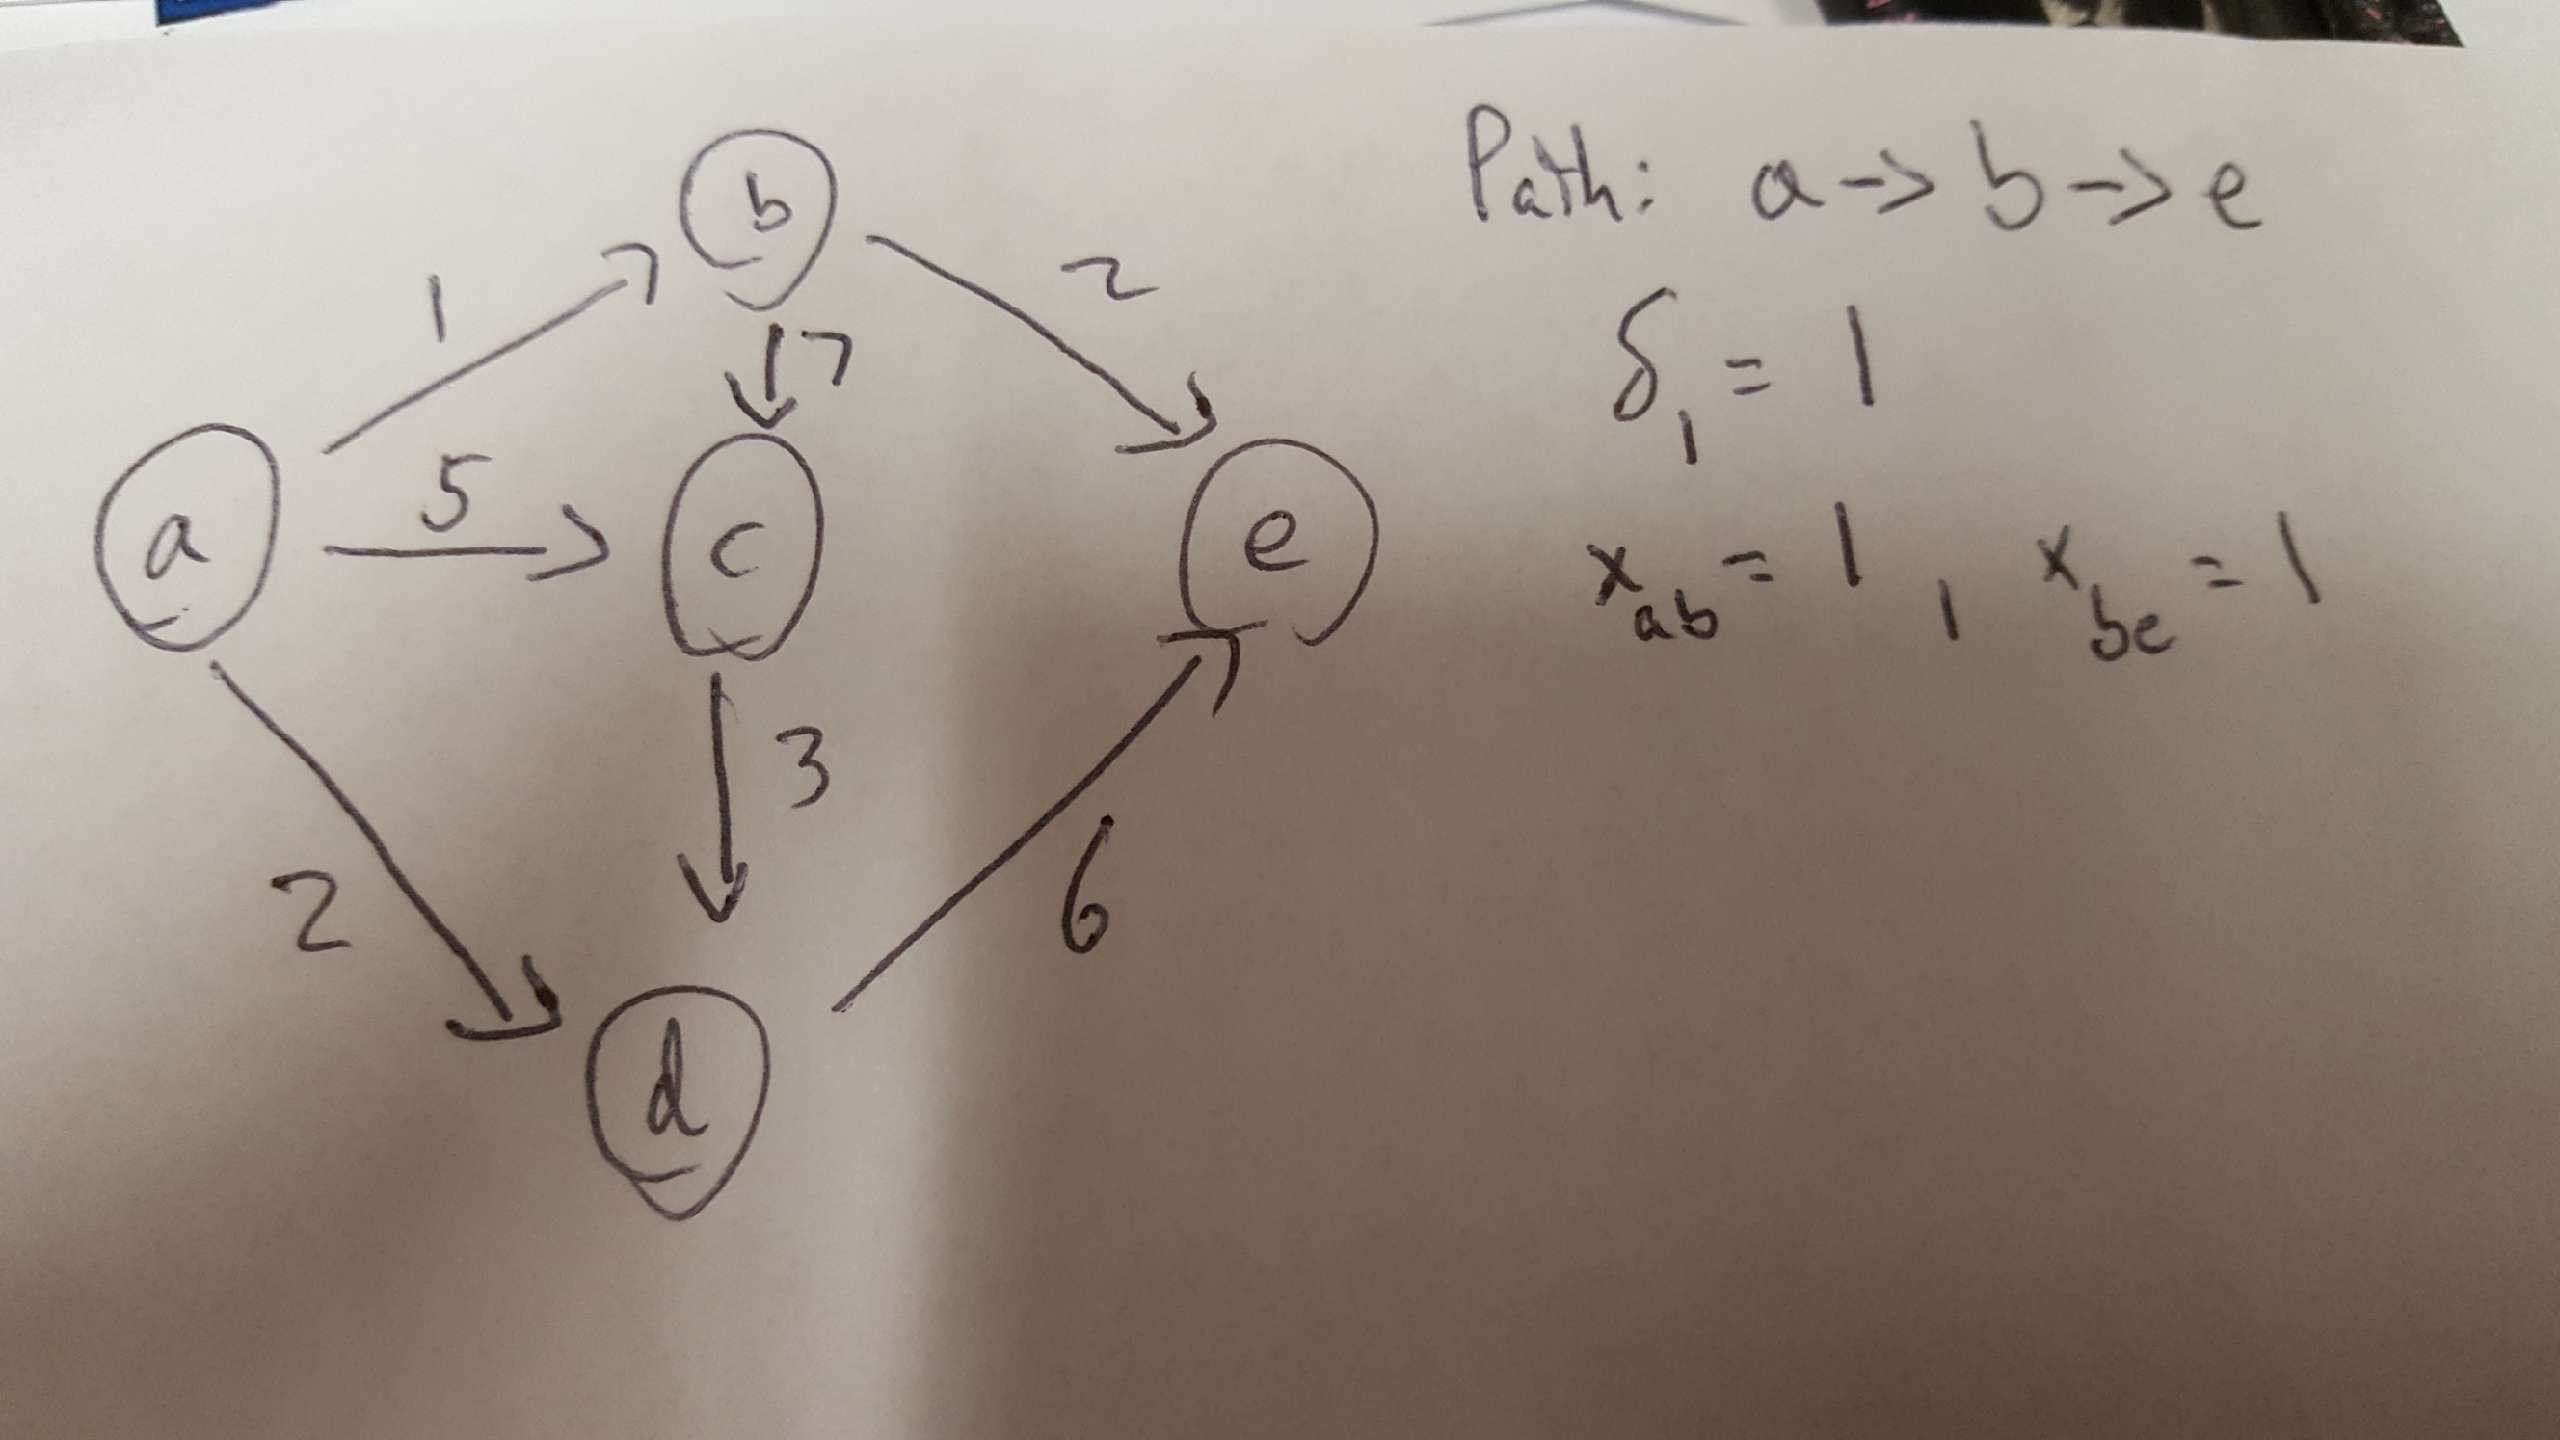
\includegraphics[width=1.0\textwidth]{FirstPath.jpeg}
\caption{ First Path }
\end{figure}
\begin{figure}[H]
\centering
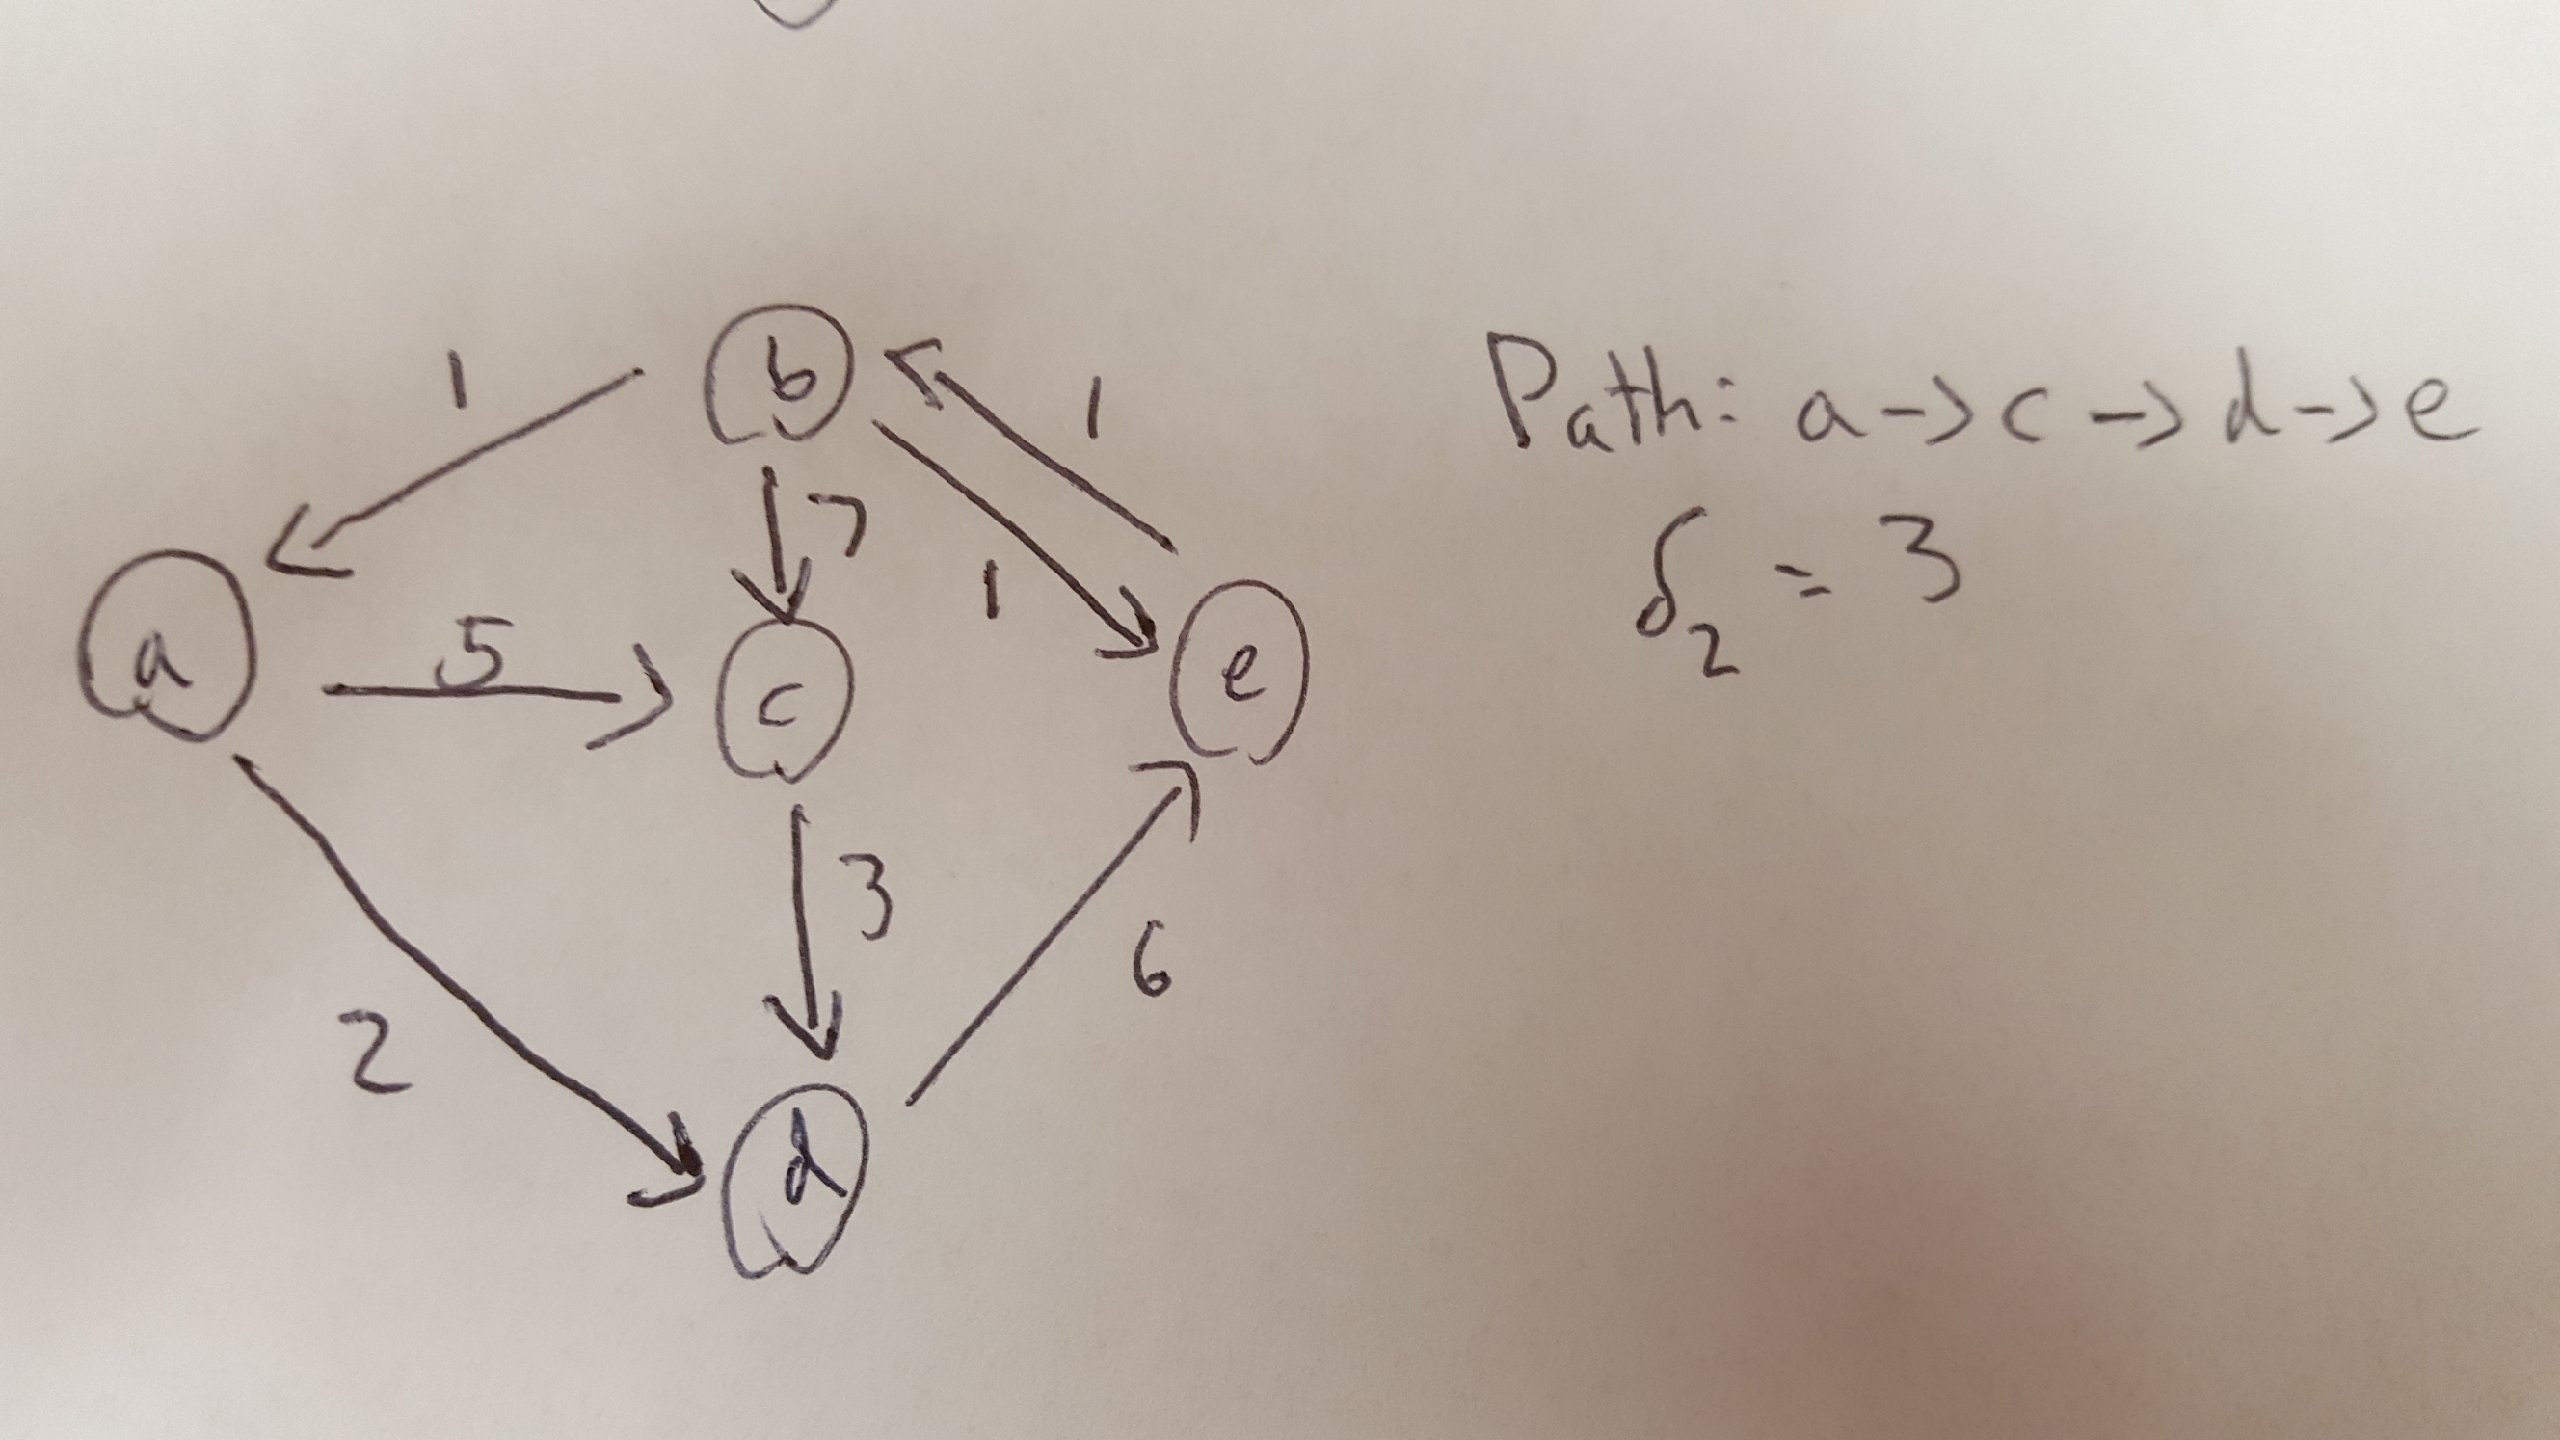
\includegraphics[width=1.0\textwidth]{SecondPath.jpeg}
\caption{ Second Path }
\end{figure}
\begin{figure}[H]
\centering
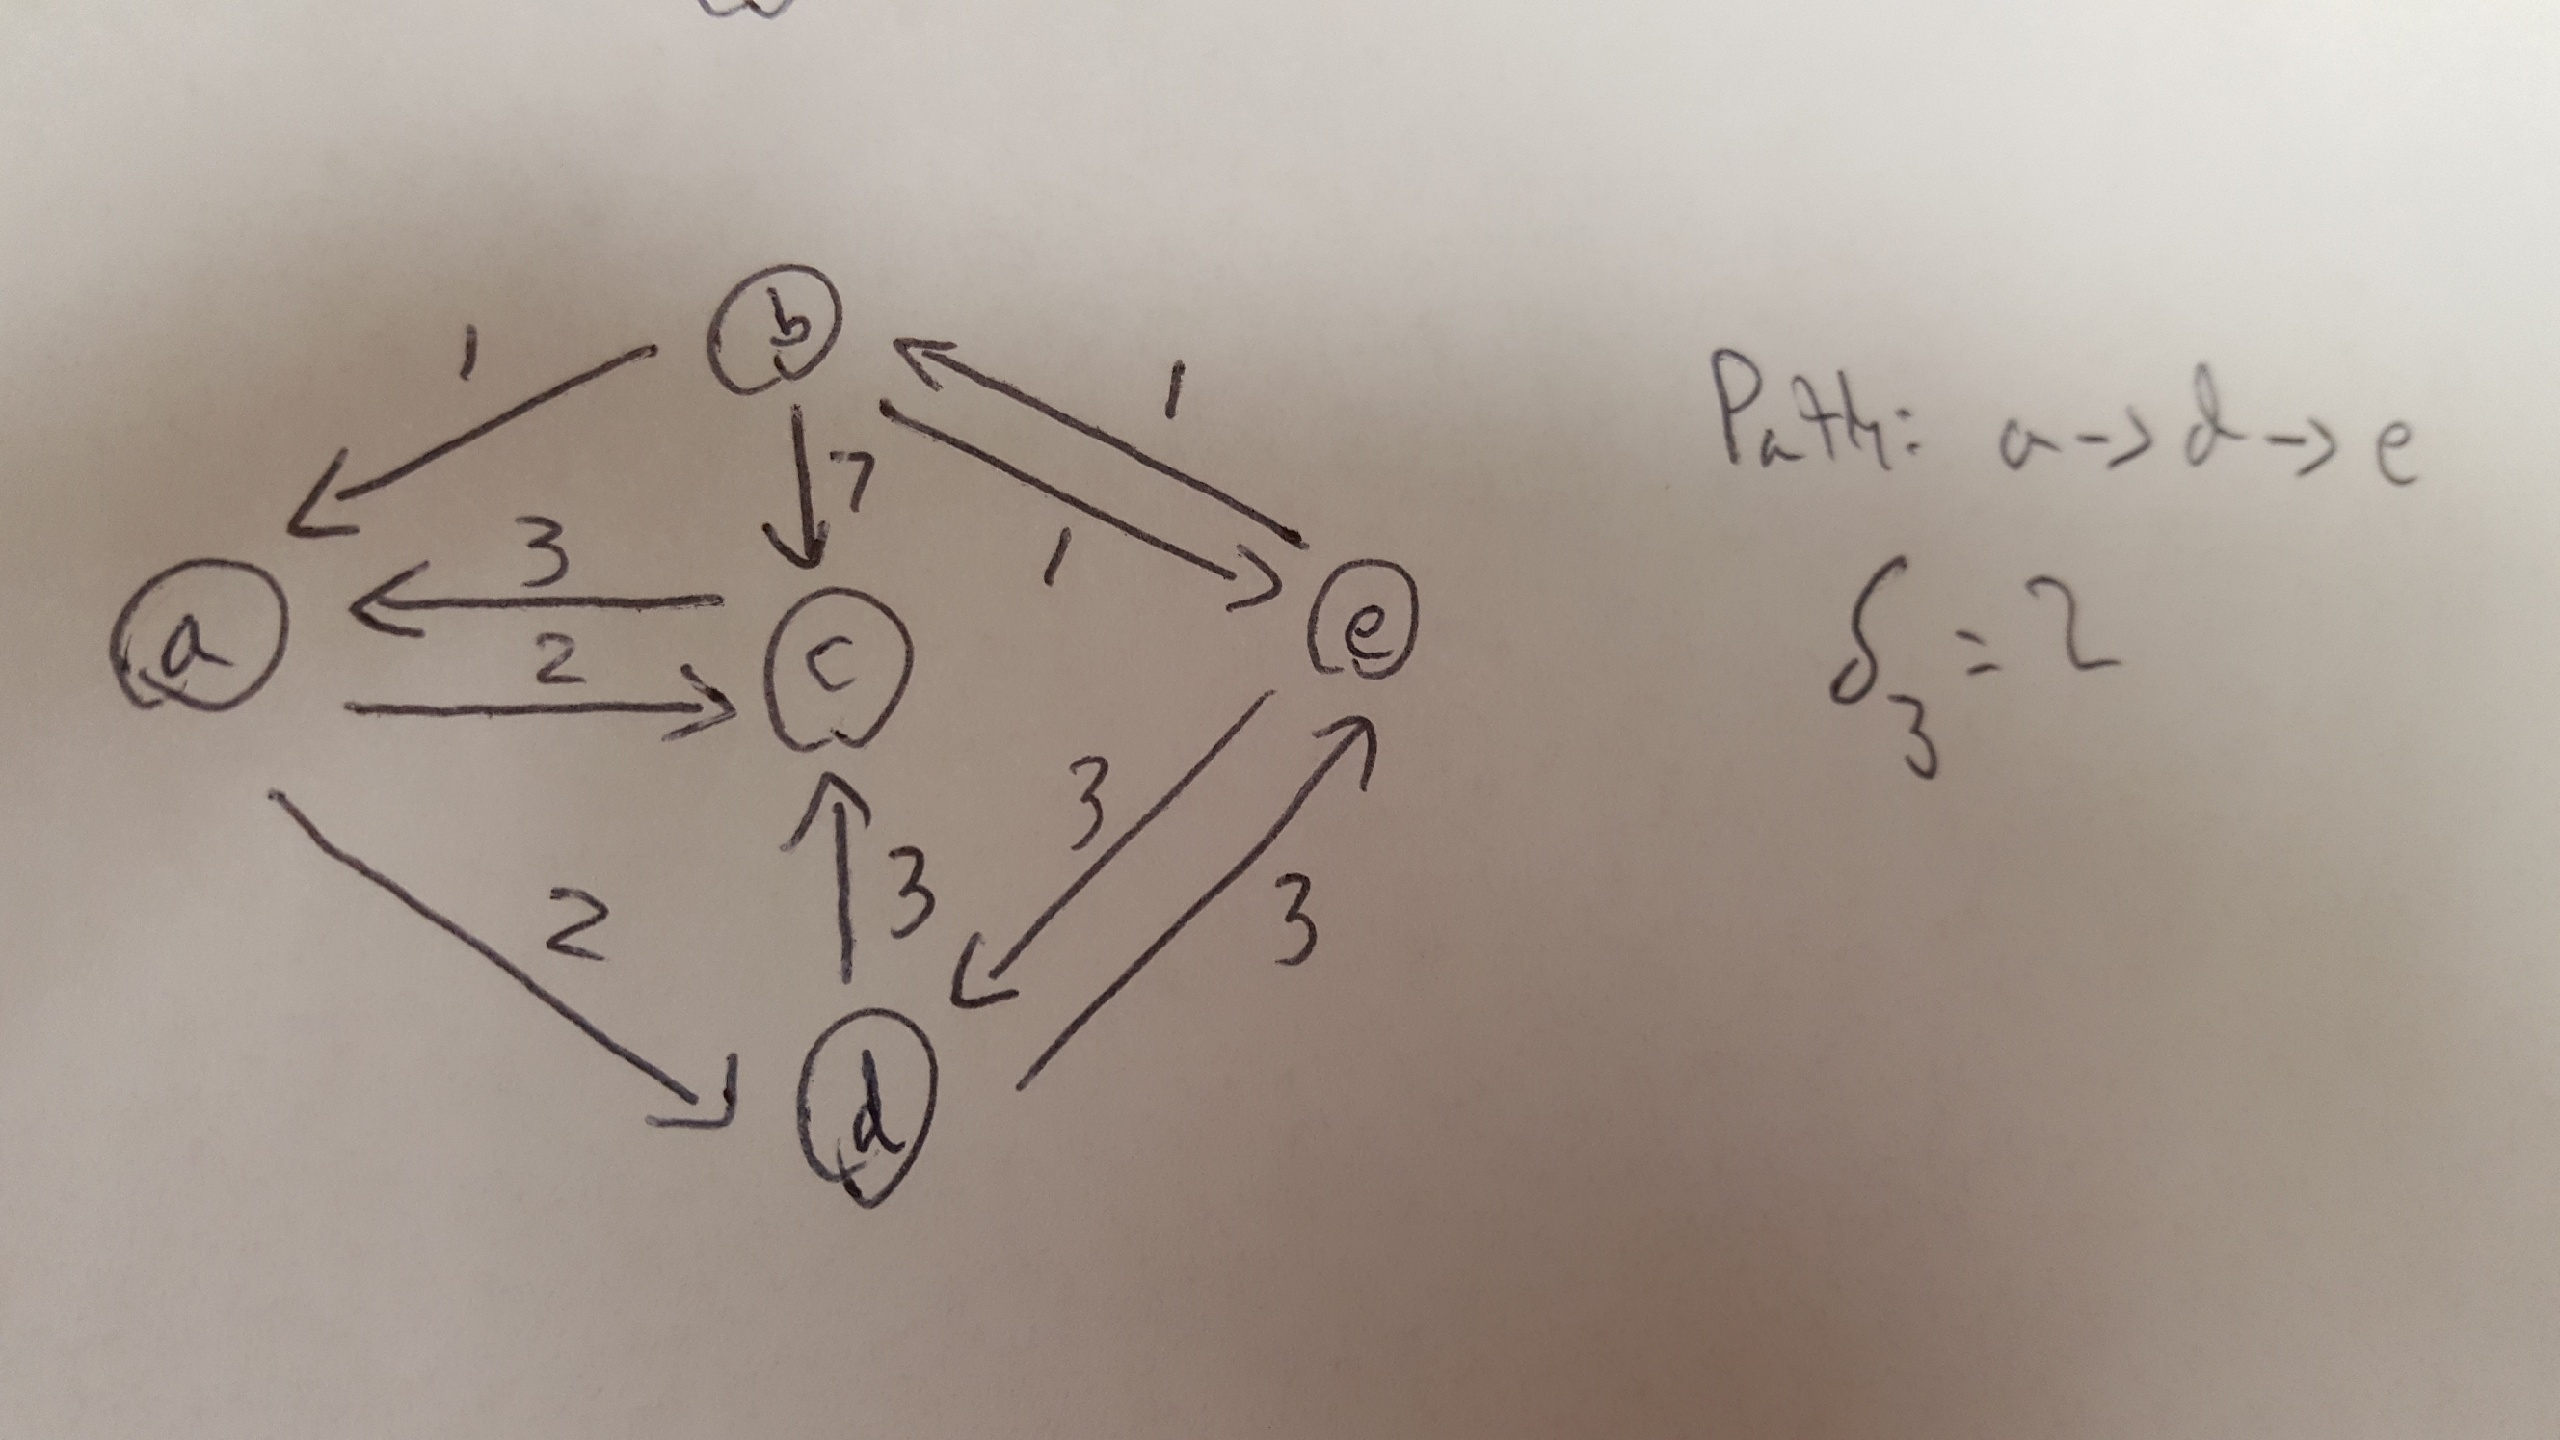
\includegraphics[width=1.0\textwidth]{ThridPath.jpeg}
\caption{ Third Path }
\end{figure}
\begin{figure}[H]
\centering
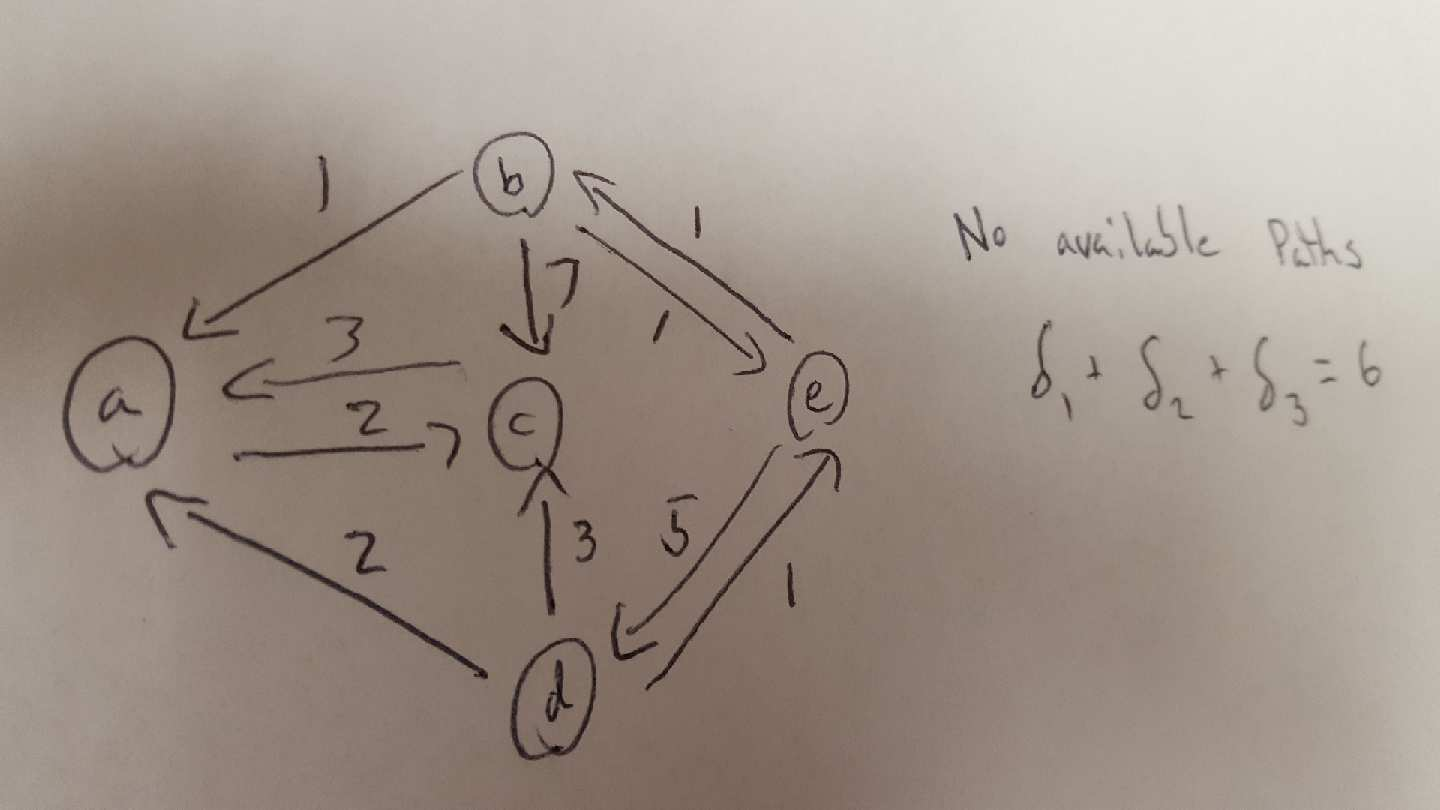
\includegraphics[width=1.0\textwidth]{FourthPath.jpeg}
\caption{ Fourth Path }
\end{figure}

This implies that the maximum flow is 6. We can verify this with the dual, and can see that the minimum cut that can be made is 6 as well.

\begin{figure}[H]
\centering
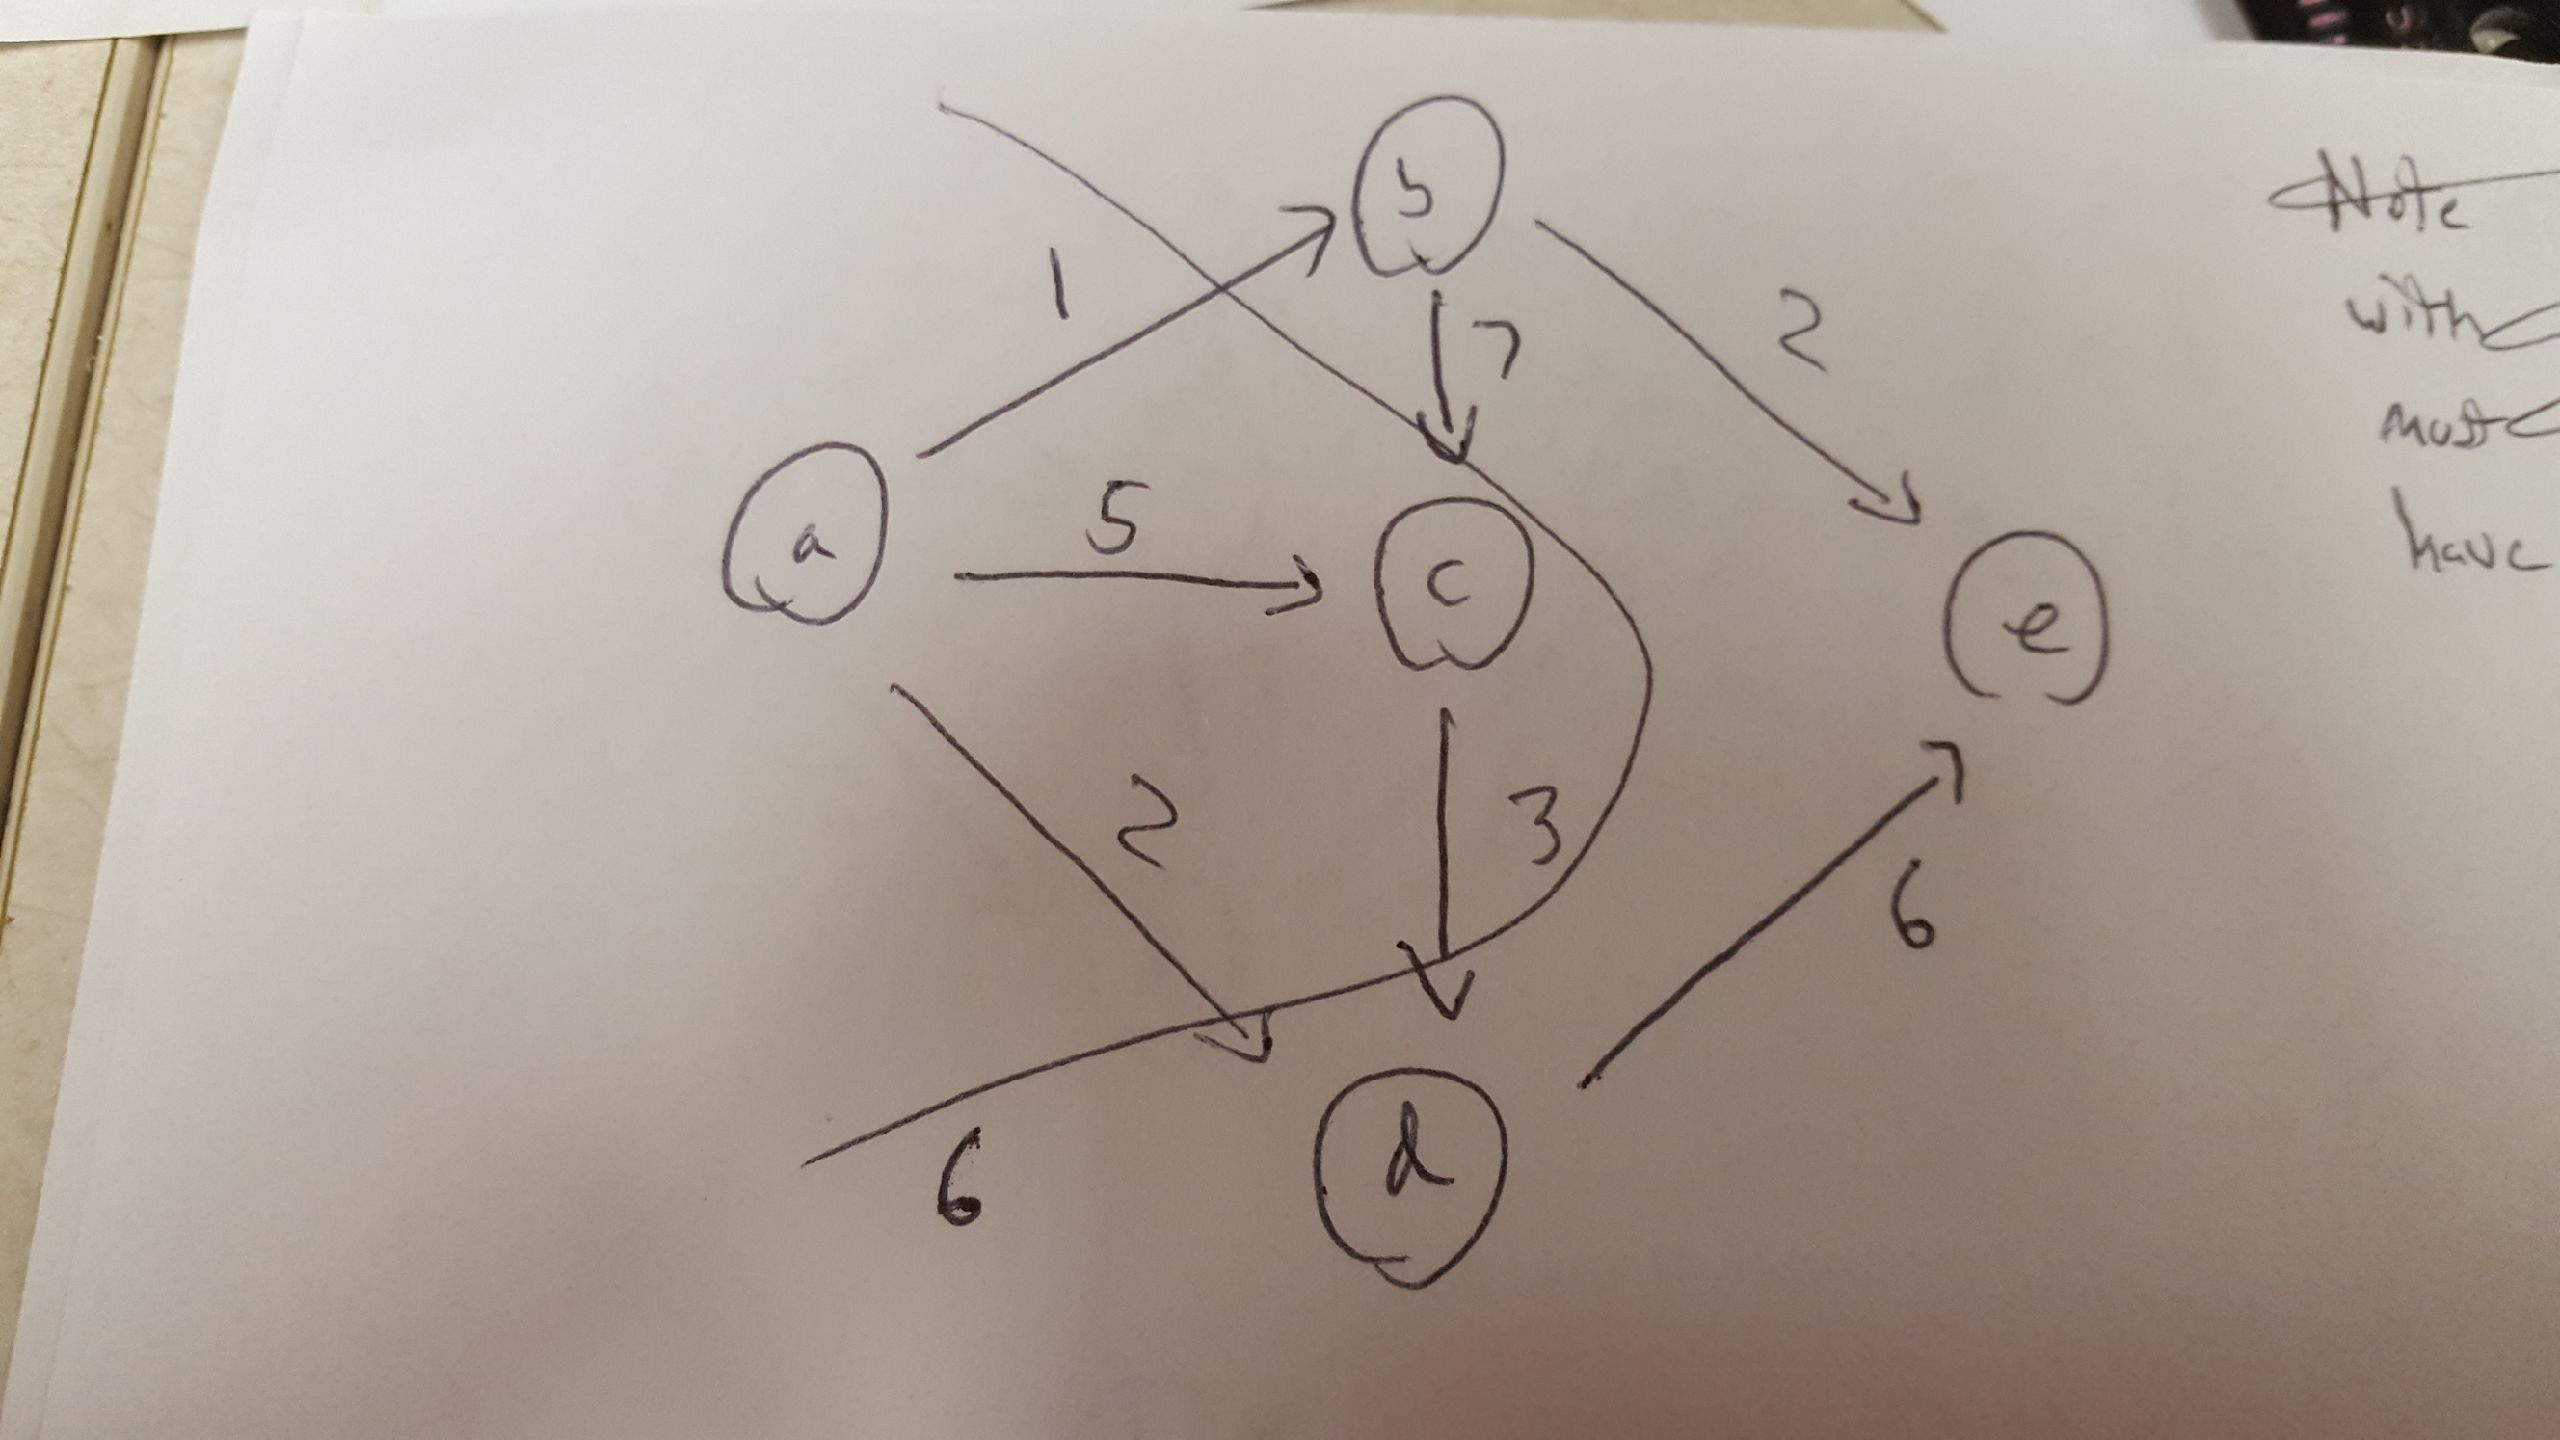
\includegraphics[width=1.0\textwidth]{Cut.jpeg}
\caption{ Minimum Cut }
\end{figure}

It is clear that no cut can be made smaller while partitioning the graph with the start in one section and the end in the other. 


\section*{Question 5.}
\subsection*{a.}
\begin{equation*}
\begin{alignedat}{3}
&\text{max }&x_1 + 3x_2&\\
&\text{s.t. } &x_1 + x_2 - e_1 &= 5\\
& &x_1 - 2x_2 + s_1  &= 2\\
& &x_1, x_2, e_1, s_1 &\geq 0
\end{alignedat}
\end{equation*}

\subsection*{b.}
\begin{equation*}
\begin{alignedat}{3}
&\text{max }&x_1 + 3x_2 -Ma_1&\\
&\text{s.t. } &x_1 + x_2 - e_1 + a_1  &= 5\\
& &x_1 - 2x_2 + s_1  &= 2\\
& &x_1, x_2, e_1, a_1, s_1 &\geq 0
\end{alignedat}
\end{equation*}

\subsection*{c.}
\[
	\left[ {\begin{array}{cccccc|c}
	Z & x_1 & x_2 & s_1 & e_1 & a_1 & RHS\\ \cline{1-7}
	1 & -1 & -3 & 0 & 0 & M & 0 \\
	0 &1 & 1 & 0 & -1 & 1 & 5\\
	0 & 1 & -2 & 1 & 0 & 0 & 2\\
	\end{array} } \right]
\]

\[
	\left[ {\begin{array}{cccccc|c}
	Z & x_1 & x_2 & s_1 & e_1 & a_1 & RHS\\ \cline{1-7}
	1 & -1 - M & -3 - M & 0 & M & 0 & -5M \\
	0 &1 & 1 & 0 & -1 & 1 & 5\\
	0 & 1 & -2 & 1 & 0 & 0 & 2\\
	\end{array} } \right]
\]

\[
	\left[ {\begin{array}{cccccc|c}
	Z & x_1 & x_2 & s_1 & e_1 & a_1 & RHS\\ \cline{1-7}
	1 & 2 & 0 & 0 & -3 & -3 + M & 15 \\
	0 & 1 & 1 & 0 & -1 & 1 & 5\\
	0 & 3 & 0 & 1 & -3 & 2 & 12\\
	\end{array} } \right]
\]

Note that we would like $e_1$ to enter the basis, but both ratios are negative, leading us to an unbounded problem.

\subsection*{d.}
Since the problem has no positive artificial variables, and the final tableau describes a point, $x_2 =5, x_1 = 0$ that is in the feasible set, the solution is feasible.
\newline
However the solution is unbounded, and its direction in the $x_1,x_2$ plane can be determined:
\begin{eqnarray*}
x_1 + x_2 - e_1 = 5 \\
3x_1 - 3e_2 = 12 \\
\end{eqnarray*}
This has a solution of $x_1 = 4 + e_1$ and $x_2 = 1$.
Our parametric solution is: $\textbf{x} = {1 \choose 4} + e_1 { 1 \choose 0 }$.
\newline
Thus the direction of unboundedness is: ${1 \choose 0 }$.


\end{document}